\let\negmedspace\undefined
\let\negthickspace\undefined
\documentclass[journal]{IEEEtran}
\usepackage[a4paper, margin=10mm, onecolumn]{geometry}
%\usepackage{lmodern} % Ensure lmodern is loaded for pdflatex
\usepackage{tfrupee} % Include tfrupee package

\setlength{\headheight}{1cm} % Set the height of the header box
\setlength{\headsep}{0mm}     % Set the distance between the header box and the top of the text

\usepackage{gvv-book}
\usepackage{gvv}
\usepackage{cite}
\usepackage{amsmath,amssymb,amsfonts,amsthm}
\usepackage{algorithmic}
\usepackage{graphicx}
\usepackage{textcomp}
\usepackage{xcolor}
\usepackage{txfonts}
\usepackage{listings}
\usepackage{enumitem}
\usepackage{mathtools}
\usepackage{gensymb}
\usepackage{comment}
\usepackage[breaklinks=true]{hyperref}
\usepackage{tkz-euclide} 
\usepackage{listings}
% \usepackage{gvv}                                        
\def\inputGnumericTable{}                                 
\usepackage[latin1]{inputenc}                                
\usepackage{color}                                            
\usepackage{array}                                            
\usepackage{longtable}                                       
\usepackage{calc}                                             
\usepackage{multirow}                                         
\usepackage{hhline}                                           
\usepackage{ifthen}                                           
\usepackage{lscape}
\usepackage{tikz}
\usetikzlibrary{patterns}
\begin{document}


\bibliographystyle{IEEEtran}
\vspace{3cm}


\numberwithin{equation}{enumi}
\numberwithin{figure}{enumi}
\renewcommand{\thetable}{\theenumi}


% Marks the beginning of the document

\bibliographystyle{IEEEtran}
\vspace{3cm}


\title{GATE ASSIGNMENT-1}
\author{AI25BTECH11004-B.JASWANTH}
% \maketitle
% \newpage
% \bigskip
{\let\newpage\relax\maketitle}


\renewcommand{\thefigure}{\theenumi}
\renewcommand{\thetable}{\theenumi}
\setlength{\intextsep}{10pt} % Space between text and floats

\section*{General Aptitude (GA)}
\begin{enumerate}[label=\textbf{Q.\arabic*.}, start=1, align=left, itemsep=2em]

% Q.1
\item ``I have not yet decided what I will do this evening; I \rule{2cm}{0.1pt} visit a friend.''\hfill(GATE ST 2023)
\begin{enumerate}
\item mite
\item would
\item might
\item didn't
\end{enumerate}


% Q2
\item Eject : Insert :: Advance : \rule{2cm}{0.1pt}\newline
(By word meaning) \hfill(GATE ST 2023)
\begin{enumerate}
    \item Advent
    \item Progress
    \item Retreat
    \item Loan
\end{enumerate}

% Q3
\item In the given figure, PQRSTV is a regular hexagon with each side of length $5\;\mathrm{cm}$. A circle is drawn with its centre at $V$ such that it passes through $P$. What is the area (in $\mathrm{cm}^2$) of the shaded region? (The diagram is representative) \hfill(GATE ST 2023)
 \begin{figure}[H]
     \centering
     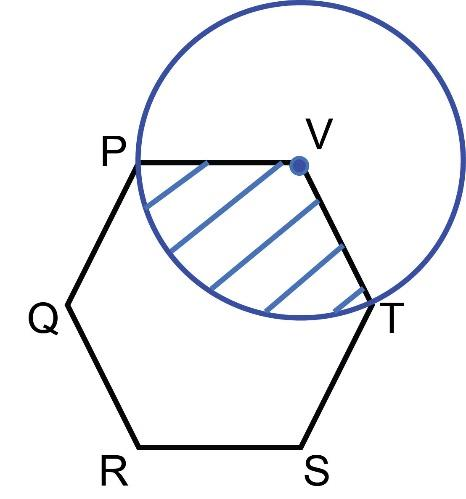
\includegraphics[width=0.5\columnwidth]{figs/Q.3image.png}
     \caption{}
     \label{fig:placeholder}
 \end{figure}
        
\begin{enumerate}
    \item  $\dfrac{25\pi}{3}$
    \item  $\dfrac{20\pi}{3}$
    \item  $6\pi$
    \item  $7\pi$
\end{enumerate}
   

% Q4
\item A duck named Donald Duck says ``All ducks always lie.''\\
Based only on the information above, which one of the following statements can be logically inferred with certainty? 
\hspace*{15.7cm}(GATE ST 2023)
\begin{enumerate}
    \item Donald Duck always lies.
    \item Donald Duck always tells the truth.
    \item Donald Duck's statement is true.
    \item Donald Duck's statement is false.
\end{enumerate}

% Q5
\item A line of symmetry is defined as a line that divides a figure into two parts in a way such that each part is a mirror image of the other part about that line.

The figure below consists of 20 unit squares arranged as shown. In addition to the given black squares, upto 5 more may be coloured black. Which one among the following options depicts the minimum number of boxes that must be coloured black to achieve two lines of symmetry? (The figure is representative) \hfill(GATE ST 2023)

    \begin{figure}[H]
        \centering
        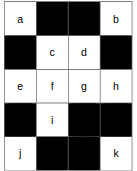
\includegraphics[width=0.5\columnwidth]{figs/Q.5image.png}
        \caption{}
        \label{fig:placeholder}
    \end{figure}
   
\begin{enumerate}
    \item d
    \item c, d, i
    \item c, i
    \item c, d, i, f, g
\end{enumerate}




% Q6
\item Based only on the truth of the statement `Some humans are intelligent', which one of the following options can be logically inferred with certainty? \hfill(GATE ST 2023)

\begin{enumerate}
    \item No human is intelligent.
    \item All humans are intelligent.
    \item Some non-humans are intelligent.
    \item Some intelligent beings are humans.
\end{enumerate}

% Q7
\item Which one of the options can be inferred about the mean, median, and mode for the given probability distribution (i.e., probability mass function), $P(x)$, of a variable $x$? \hfill(GATE ST 2023)\\

    \begin{figure}[h]
        \centering
        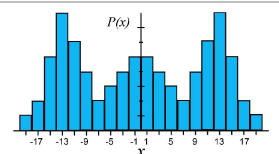
\includegraphics[width=0.5\columnwidth]{figs/Q.7image.png}        
        \label{fig:placeholder}
    \end{figure}
    
\begin{enumerate}
    \item mean $=$ median $\neq$ mode
    \item mean $=$ median $=$ mode
    \item mean $\neq$ median $=$ mode
    \item mean $\neq$ mode $=$ median
\end{enumerate}

% Q8
\item The James Webb telescope, recently launched in space, is giving humankind unprecedented access to the depths of time by imaging very old stars formed almost 13 billion years ago. Astrophysicists and cosmologists believe that this odyssey in space may even shed light on the existence of dark matter. Dark matter is supposed to interact only via the gravitational interaction and not through the electromagnetic-, the weak- or the strong-interaction. This may justify the epithet ``dark'' in dark matter.

Based on the above paragraph, which one of the following statements is FALSE? \hfill(GATE ST 2023)

\begin{enumerate}
    \item No other telescope has captured images of stars older than those captured by the James Webb telescope.
    \item People other than astrophysicists and cosmologists may also believe in the existence of dark matter.
    \item The James Webb telescope could be of use in the research on dark matter.
    \item If dark matter was known to interact via the strong-interaction, then the epithet ``dark'' would be justified.
\end{enumerate}

% Q9
\item Let $a = 30!$, $b = 50!$, and $c = 100!$. Consider the following numbers:
$\log_a c,\; \log_c a,\; \log_b a,\; \log_a b$.\newline
Which one of the following inequalities is CORRECT? \hfill(GATE ST 2023)

\begin{enumerate}
    \item $\log_c a < \log_b a < \log_a b < \log_a c$
    \item $\log_c a < \log_a b < \log_b a < \log_b c$
    \item $\log_c a < \log_b a < \log_a c < \log_a b$
    \item $\log_b a < \log_c a < \log_a b < \log_a c$
\end{enumerate}

% Q10
\item A square of side length $4\;\mathrm{cm}$ is given. The boundary of the shaded region is defined by one semi-circle on the top and two circular arcs at the bottom, each of radius $2\;\mathrm{cm}$, as shown.
The area of the shaded region is \rule{3cm}{0.1pt} cm$^2$.\hfill(GATE ST 2023)
    \begin{figure}[H]
        \centering
        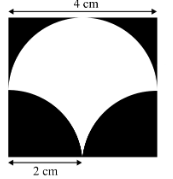
\includegraphics[width=0.5\columnwidth]{figs/Q.10image.png}
        \label{fig:placeholder}
    \end{figure}
\begin{enumerate}
    \item 8
    \item 4
    \item 12
    \item 10
\end{enumerate}

\end{enumerate}

% Continue similarly for the rest of the questions: Q11–Q65
% For numerical answers, use: \textbf{Q.n}. [Statement] (rounded off to two decimal places) equals \underline{\hspace{3cm}}
\begin{enumerate}[label=\textbf{Q.\arabic*.}, start=11, align=left, itemsep=2em]

% Q11
\item The area of the region bounded by the parabola $x = -y^2$ and the line $y = x + 2$ equals \hfill(GATE ST 2023) 
\begin{enumerate}
    \item $\frac{3}{2}$
    \item $\frac{7}{2}$
    \item $\frac{9}{2}$
    \item $9$
\end{enumerate}

% Q12
\item Let $A$ be a $3 \times 3$ real matrix having eigenvalues $1, 0, -1$. If $B = A^2 + 2A + I_3$, where $I_3$ is the $3\times 3$ identity matrix, then which one of the following statements is true? \hfill(GATE ST 2023) 
\begin{enumerate}
    \item $B^3 - 5B^2 + 4B = 0$
    \item $B^3 - 5B^2 - 4B = 0$
    \item $B^3 + 5B^2 - 4B = 0$
    \item $B^3 + 5B^2 + 4B = 0$
\end{enumerate}

% Q13
\item Consider the following statements: 

(I) Let $A$ and $B$ be two $n\times n$ real matrices. If $B$ is invertible, then $\mathrm{rank}(BA) = \mathrm{rank}(A)$.

(II) Let $A$ be an $n\times n$ real matrix. If $A^2 \mathbf{x} = \mathbf{b}$ has a solution for every $\mathbf{b} \in \mathbb{R}^n$, then $A\mathbf{x} = \mathbf{b}$ also has a solution for every $\mathbf{b} \in \mathbb{R}^n$.

Which of the above statements is/are true? \hfill(GATE ST 2023) 
\begin{enumerate}
    \item Only (I)
    \item Only (II)
    \item Both (I) and (II)
    \item Neither (I) nor (II)
\end{enumerate}

% Q14
\item Consider the probability space $(\Omega, \mathcal{G}, P)$, where $\Omega = [0,2]$ and $\mathcal{G} = \{\varnothing, \Omega, [0,1], (1,2]\}$.  
Let $X$ and $Y$ be two functions on $\Omega$ defined as and 

\begin{align}
X(\omega) &= 
\begin{cases}
1, & \omega \in [0,1] \\
2, & \omega \in (1,2]
\end{cases} \\
Y(\omega) &= 
\begin{cases}
2, & \omega \in [0,1.5] \\
3, & \omega \in (1.5,2]
\end{cases}
\end{align}
Then which one of the following statements is true?  \hfill(GATE ST 2023)
\begin{enumerate}
    \item $X$ is a random variable with respect to \ $\mathcal{G}$, but $Y$ is not a random variable with respect to  \ $\mathcal{G}$
    \item $Y$ is a random variable with respect to \ $\mathcal{G}$, but $X$ is not a random variable with respect to  \ $\mathcal{G}$  
    \item Neither $X$ nor $Y$ is a random variable with respect to \ $\mathcal{G}$  
    \item Both $X$ and $Y$ are random variables with respect to \ $\mathcal{G}$
\end{enumerate}

% Q15
\item Let $\Phi(\cdot)$ denote the cumulative distributive function of a standard normal random variable. If the random variable X has the cumulative distribution function  
\[
F(x) =
\begin{cases}
\Phi(x) & x < -1 \\
\Phi(x + 1) & x \ge -1
\end{cases}
\]
then which one of the following statements is true? \hfill(GATE ST 2023) 
\begin{enumerate}[label=(\Alph*)]
    \item $P(X \le -1) = \frac{1}{2}$
    \item $P(X = -1) = \frac{1}{2}$
    \item $P(X < -1) = \frac{1}{2}$
    \item $P(X \le 0) = \frac{1}{2}$
\end{enumerate}

% Q16
\item Let $X$ be a random variable with probability density function
\[ f(x) = \begin{cases}
\alpha \lambda x^{\alpha - 1} e^{ - \lambda x^{\alpha}}, & x>0 \\
0, & \text{otherwise}
\end{cases} \]
where $\alpha > 0$and $\lambda > 0$. If the median of $X$ is $1$ and the third quantile is $2$, then $(\alpha, \lambda)$ equals \hfill(GATE ST 2023) 
\begin{enumerate}
    \item $(1, \log_e 2)$
    \item $(1, 1)$
    \item $(2, \log_e 2)$image
    \item $(1, \log_e 3)$
\end{enumerate}

% Q17
\item Let $X$ be a random variable having poission distribution with mean $\lambda > 0$. Then $E\left( \frac{1}{X+1} \,\middle|\, X > 0\right)$ equals  \hfill(GATE ST 2023)
\begin{enumerate}
    \item $\frac{1 - e^{-\lambda} - \lambda e^{-\lambda}}{\lambda (1 - e^{-\lambda})}$
    \item $\frac{1 - e^{-\lambda}}{\lambda}$
    \item $\frac{1 - e^{-\lambda} - \lambda e^{-\lambda}}{\lambda}$
    \item $\frac{1 - e^{-\lambda}}{\lambda + 1}$
\end{enumerate}

% Q18
\item Suppose that $X$ has the probability density function
\[ f(x) = \begin{cases}
\frac{\lambda^\alpha}{\Gamma(\alpha)} x^{\alpha - 1} e^{-\lambda x}, & x>0 \\
0, & \text{otherwise}
\end{cases} \]
where $\alpha > 0$ and $\lambda > 0$. Which one of the following statements is NOT true? \hfill(GATE ST 2023) 
\begin{enumerate}
    \item $E(X)$ exists for all $\alpha > 0$ and $\lambda > 0$
    \item Variance of X exists for all $\alpha > 0$ and $\lambda > 0$
    \item $E(1/X)$ exists for all $\alpha > 0$ and $\lambda > 0$
    \item $E(\log_e(1+X))$ exists for all $\alpha > 0$ and $\lambda > 0$
\end{enumerate}

% Q19
\item Let $(X,Y)$ have joint probability density function
\[ f(x,y) = \begin{cases}
8xy, & 0 < x < y < 1 \\
0, & \text{otherwise}
\end{cases} \]
If $E(X \mid Y = y_0) = \frac12$, then $y_0$ equals \hfill(GATE ST 2023) 
\begin{enumerate}
    \item $\frac{3}{4}$
    \item $\frac{1}{2}$
    \item $\frac{1}{3}$
    \item $\frac{2}{3}$
\end{enumerate}

% Q20
\item Suppose there are $5$ boxes, each containing $3$ blue pens, $1$ red pen, and $2$ black pens. One pen is drawn at random from each of these 5 boxes.If the random variable $X_1$ denotes the total number of blue pens drawn and the random variable $X_2$ denotes the total  number of red pens drawn, Then $P(X_1 = 2, X_2 = 1)$ equals  \hfill(GATE ST 2023)
\begin{enumerate}
    \item $\frac{5}{36}$
    \item $\frac{5}{18}$
    \item $\frac{5}{12}$
    \item $\frac{5}{9}$
\end{enumerate}

% Q21  
\item Let $\{X_n\}_{n \geq 1}$ and $\{Y_n\}_{n \geq 1}$ be two sequences of random variables and $X$ and $Y$ be two random variables, all of them defined on the same probability space. Which one of the following statements is true?\hfill(GATE ST 2023)

\begin{enumerate}
    \item If $\{X_n\}_{n \geq 1}$ converges in distribution to a real constant $c$, then $\{X_n\}_{n \geq 1}$ converges in probability to $c$.
    
    \item If $\{X_n\}_{n \geq 1}$ converges in probability to $X$, then $\{X_n\}_{n \geq 1}$ converges in 3rd mean to $X$.
    
    \item If $\{X_n\}_{n \geq 1}$ converges in distribution to $X$ and $\{Y_n\}_{n \geq 1}$ converges in distribution to $Y$, then $\{X_n + Y_n\}_{n \geq 1}$ converges in distribution to $X + Y$.
    
    \item If $\{E(X_n)\}_{n \geq 1}$ converges to $E(X)$, then $\{X_n\}_{n \geq 1}$ converges in 1st mean to $X$.
\end{enumerate}

% Q22
\item Let $X$ be a random variable with probability density function
\[ f(x;\lambda) = \begin{cases}
\frac{1}{\lambda} e^{-x/\lambda}, & x>0 \\
0, & \text{otherwise}
\end{cases} \]
where $\lambda > 0$ is an unknown parameter. Let $Y_1,\dots,Y_n$ be a random sample of size n from a population having the same distribution as $X^2$.\\
If $\overline{Y} = \frac1n \sum_{i=1}^n Y_i$, then which one of the following statements is true?  \hfill(GATE ST 2023)
\begin{enumerate}
    \item $\sqrt{\overline{Y}/2}$ is a method of moments estimator of $\lambda$
    \item $\sqrt{\overline{Y}}$ is a method of moments estimator of $\lambda$
    \item $\frac{1}{2}\sqrt{\overline{Y}}$ is a method of moments estimator of $\lambda$
    \item $2\sqrt{\overline{Y}}$ is a method of moments estimator of $\lambda$
\end{enumerate}

% Q23
\item Let $X_1,\dots,X_n$ be a random sample of size n$(\geq 2)$ from a population having probability density function
\[ f(x;\theta) = \begin{cases}
\frac{2}{\theta x (-\ln x)} e^{ - \frac{(\ln x)^2}{\theta}}, & 0 < x < 1 \\
0, & \text{otherwise}
\end{cases} \]
where $\theta >0$ is an unknown parameter.Then which one of the following statements is true?\hfill(GATE ST 2023)  
\begin{enumerate}
    \item $\frac{1}{n} \sum_{i=1}^n (\ln X_i)^2$ is the maximum likelihood estimator of $\theta$  
    \item $\frac{1}{n-1} \sum_{i=1}^n (\ln X_i)^2$ is the maximum likelihood estimator of $\theta$   
    \item $\frac{1}{n} \sum_{i=1}^n \ln X_i$ is the maximum likelihood estimator of $\theta$    
    \item $\frac{1}{n-1} \sum_{i=1}^n \ln X_i$ is the maximum likelihood estimator of $\theta$   
\end{enumerate}

% Q24
\item Let $X_1$,$X_2$,.....,$X_n$ be a random Sample of size n from a population having uniform distribution over the interval $(1/3,\theta)$,where $\theta>1/3$ is an unknown parameter.If $Y$= max\{$X_1$,$X_2$,....$X_n$\},then Which one of the following statements is true?\hfill(GATE ST 2023)  
\begin{enumerate}
    \item $\left( \frac{n+1}{n} \right) (Y - \frac13) + \frac13$ is an unbiased estimator 0f $\theta$  
     \item $\left( \frac{n}{n+1} \right) (Y - \frac13) + \frac13$  is an unbiased estimator 0f $\theta$  
    \item $\left( \frac{n+1}{n} \right) (Y + \frac13) - \frac13$ is an unbiased estimator 0f $\theta$   
    \item $Y$ is an unbiased estimator 0f $\theta$  
\end{enumerate}

% Q25
\item Suppose that $X_1, X_2, \dots, X_n, Y_1, Y_2, \dots, Y_n$ are independent and identically
distributed random vectors each having $N_p(\mu, \Sigma)$ distribution, where $\Sigma$ is non-singular, $p>1$ and $n>1$. 
If 
\[
\overline{X} = \frac{1}{n} \sum_{i=1}^n X_i, 
\quad
\overline{Y} = \frac{1}{n} \sum_{i=1}^n Y_i,
\]
then which one of the following statements is true?\hfill(GATE ST 2023)
\begin{enumerate}
    \item There exists $c>0$ such that $c\, (\overline{X} - \mu)^{\top} \Sigma^{-1} (\overline{X} - \mu)$ has $\chi^2$ distribution with $p$ degrees of freedom
    \item There exists $c>0$ such that $c\, (\overline{X} - \overline{Y})^{\top} \Sigma^{-1} (\overline{X} - \overline{Y})$ has $\chi^2$ distribution with $(p-1)$ degrees of freedom
    \item There exists $c>0$ such that $c \sum_{i=1}^n (X_i - \overline{X})^{\top} \Sigma^{-1} (X_i - \overline{X})$ has $\chi^2$ distribution with $p$ degrees of freedom
    \item There exists $c>0$ such that $c \sum_{i=1}^n (X_i - Y_i - \overline{X} + \overline{Y})^{\top} \Sigma^{-1} (X_i - Y_i - \overline{X} + \overline{Y})$ has $\chi^2$ distribution with $p$ degrees of freedom
\end{enumerate}

% Q26  
\item Consider the following regression model  
\[
y_k = \alpha_0 + \alpha_1 \log_e k + \epsilon_k, \quad k = 1, 2, \dots, n,
\]
where $\epsilon_k$'s are independent and identically distributed random variables each having probability density function  
\[
f(x) = \frac{1}{2} e^{-|x|}, \quad x \in \mathbb{R}.
\]
Then which one of the following statements is true? \hfill(GATE ST 2023) 

\begin{enumerate}
    \item The maximum likelihood estimator of $\alpha_0$ does not exist
    \item The maximum likelihood estimator of $\alpha_1$ does not exist
    \item The least squares estimator of $\alpha_0$ exists and is unique
    \item The least squares estimator of $\alpha_1$ exists, but it is not unique
\end{enumerate}


% Q27 
S\item uppose that $X_1, X_2, \dots, X_n$ are independent and identically distributed random 
variables each having probability density function $f(\cdot)$ and median $\theta$.  
We want to test
\[
H_0: \theta = \theta_0 \quad \text{against} \quad H_1: \theta > \theta_0.
\]
Consider a test that rejects $H_0$ if $S > c$ for some $c$ depending on the size of 
the test, where $S$ is the cardinality of the set $\cbrak{i : X_i > \theta_0, \; 1 \le i \le n }$.  
Then which one of the following statements is true? \hfill(GATE ST 2023) 

\begin{enumerate}
    \item Under $H_0$, the distribution of $S$ depends on $f(\cdot)$
    \item Under $H_1$, the distribution of $S$ does not depend on $f(\cdot)$
    \item The power function depends on $\theta$
    \item The power function does not depend on $\theta$
\end{enumerate}

% Q28  
\item Suppose that $x$ is an observed sample of size $1$ from a population with 
probability density function $f(\cdot)$. Based on $x$, consider testing 
\[
H_0: f(y) = \frac{1}{\sqrt{2\pi}} e^{-y^2/2}, \quad y \in \mathbb{R} 
\quad \text{against} \quad 
H_1: f(y) = \frac12 e^{-|y|}, \quad y \in \mathbb{R}.
\]
Then which one of the following statements is true?\hfill(GATE ST 2023)  

\begin{enumerate}
    \item The most powerful test rejects $H_0$ if $|x| > c$ for some $c>0$
    \item The most powerful test rejects $H_0$ if $|x| < c$ for some $c>0$
    \item The most powerful test rejects $H_0$ if $\big||x| - 1\big| > c$ for some $c>0$
    \item The most powerful test rejects $H_0$ if $\big||x| - 1\big| < c$ for some $c>0$
\end{enumerate}


% Q29
\item Let $f: \mathbb{R}^2 \to \mathbb{R}$ be defined by $f(x, y) = xy$.  
Then the maximum value (rounded off to two decimal places) of $f$ on the ellipse  
\begin{align}
x^2 + 2y^2 &= 1
\end{align}
equals \underline{\hspace{2cm}}.\hfill(GATE ST 2023)


% Q30
\item Let $A$ be $2\times 2$ real matrix such that $AB=BA$ for all $2\times2$ real $B$. If $\mathrm{trace}(A)$ equals $5$, then $\det(A)$ (rounded off to two decimal places) equals \underline{\hspace{3cm}}\hfill(GATE ST 2023)



% Q31
\item Two defective bulbs are present in a set of five bulbs. To remove the two defective bulbs, the bulbs are chosen randomly one by one and tested. If $X$ denotes the minimum number of bulbs that must be tested to find out the two defective bulbs, then $P(X=3)$ (rounded off to two decimal places) equals \underline{\hspace{3cm}}\hfill(GATE ST 2023)

% Q32
\item Let $\{X_n\}_{n\ge 1}$ be a sequence of independent and identically distributed random variables each having mean $4$ and variance $9$. If 
\[
Y_n = \frac{1}{n} \sum_{i=1}^n X_i, \quad n \ge 1,
\]
then $\lim_{n\to\infty} E\left[ \left( \frac{Y_n - 4}{\sqrt{n}} \right)^2 \right]$ (in integer) equals \underline{\hspace{3cm}}\hfill(GATE ST 2023)

% Q33
\item Let $\{W_t\}_{t\ge 0}$ be a standard Brownian motion. Then $E(W_4^2 \mid W_2 = 2)$ (in integer) equals \underline{\hspace{3cm}}
\hfill(GATE ST 2023)

% Q34
\item Let $\{X_n\}_{n\ge 1}$ be a Markov chain with state space $\{1,2,3\}$ and transition probability matrix
\[
\myvec{
1/2 & 1/4 & 1/4 \\
1/3 & 1/3 & 1/3 \\
0 & 1/2 & 1/2
}
\]


Then $P(X_2 = 1 \mid X_1 = 1, X_3 = 2)$ (rounded off to two decimal places) equals \underline{\hspace{3cm}}\hfill(GATE ST 2023)

% Q35
\item Suppose $(X_1, X_2, X_3) has N_3(\mu, \Sigma)$ distribution with $\mu = (0,0,0)^\top$ and
\[
\Sigma =
\myvec{
2 & 2 & 1 \\
2 & 5 & 1 \\
1 & 1 & 1
}
\]
Given that $\Phi(-0.5) = 0.3085$, where $\Phi(\cdot)$ denotes the cumulative distributive function of a standard normal random variable,\\

$P\left( (X_1 - 2X_2 + 2X_3)^2 < \frac{7}{2} \right)$ (rounded off to two decimal places) equals \underline{\hspace{3cm}}\hfill(GATE ST 2023)


% Q36
\item Let $A$ be an $n\times n$ real matrix. Consider the following statements: 

(I) If $A$ is symmetric, then there exists $c \ge 0$ such that $A + c I_n$ is symmetric and positive definite,where $I_n$ is the $n\times n$ identity matrix. 

(II) If $A$ is symmetric and positive definite, then there exists a symmetric and positive definite $B$ such that $A = B^2$. 

Which of the above statements is/are true?\hfill(GATE ST 2023)
\begin{enumerate}
\item Only (I)
\item Only (II)
\item Both (I) and (II)
\item Neither (I) nor (II)
\end{enumerate}

% Q.37  
\item Let $X$ be a random variable with probability density function  
\[
f(x) =
\begin{cases}
\dfrac{1}{x^{2}}, & \text{if } x \ge 1, \\
0, & \text{otherwise}.
\end{cases}
\]
If $Y = \log_{e} X$, then $P\big(Y < 1 \,\big|\, Y < 2\big)$ equals  \hfill(GATE ST 2023)

\begin{enumerate}
    \item $\dfrac{e}{1+e}$
    \item $\dfrac{e^{-1}}{e+1}$
    \item $\dfrac{1}{1+e}$
    \item $\dfrac{1}{e-1}$
\end{enumerate}


% Q38
\item Let $\{N(t)\}_{t\ge0}$ be a Poisson process with rate 1.Consider the following statements.\\

(I) $P(N(3)=3 \mid N(5)=5) = {5\choose3} (3/5)^3 (2/5)^2$.  

(II) If $S_5$ denotes the time of the occurence of the 5th event for the above poission process, then $E(S_5 \mid N(5)=3) = 7$.

Which of the above statements is/are true?\hfill(GATE ST 2023)
\begin{enumerate}
\item Only (I)
\item Only (II)
\item Both (I) and (II)
\item Neither (I) nor (II)
\end{enumerate}

% Q.39  
\item Let $X_1, X_2, \dots, X_n$ be a random sample of size $n$ from a population having 
probability density function  
\[
f(x; \mu) = 
\begin{cases} 
e^{-(x-\mu)}, & \text{if } \mu \le x < \infty, \\
0, & \text{otherwise},
\end{cases}
\]
where $\mu \in \mathbb{R}$ is an unknown parameter.  
If $\hat{M}$ is the maximum likelihood estimator of the median of $X_1$,  
then which one of the following statements is true?  \hfill(GATE ST 2023)

\begin{enumerate}
    \item $P(\hat{M} \le 2) = 1 - e^{-n(1 - \log_e 2)} \quad \text{if } \mu = 1$
    \item $P(\hat{M} \le 1) = 1 - e^{-n \log_e 2} \quad \text{if } \mu = 1$
    \item $P(\hat{M} \le 3) = 1 - e^{-n(1 - \log_e 2)} \quad \text{if } \mu = 1$
    \item $P(\hat{M} \le 4) = 1 - e^{-n(2\log_e 2 - 1)} \quad \text{if } \mu = 1$
\end{enumerate}


% Q40
\item Let $X_1$,$X_2$,......,$X_10$ be a random sample of size 10 from a population having $N(0,\theta^2)$ distribution, where $\theta >0$ is an unknown parameter. 
Let $T = \frac1{10} \sum_{i=1}^{10} X_i^2$. If the mean square error of $cT$($c>0$),as an estimator of $\theta^2$),is minimized at $c=c_0$,then the value of $c_0$ equals\hfill(GATE ST 2023)

\begin{enumerate}
\item $\frac{5}{6}$
\item $\frac{2}{3}$
\item $\frac{3}{5}$
\item $\frac{1}{2}$
\end{enumerate}

% Q41
\item Suppose that $\mathbf{X}_1, \mathbf{X}_2, \dots, \mathbf{X}_{10}$ are independent and identically distributed random 
vectors each having $N_2(\boldsymbol{\mu}, \Sigma)$ distribution, where $\Sigma$ is non-singular.  
If  
\[
U = \frac{1}{1 + (\bar{\mathbf{X}} - \boldsymbol{\mu})^{T} \Sigma^{-1} (\bar{\mathbf{X}} - \boldsymbol{\mu})},
\]
where  
\[
\bar{\mathbf{X}} = \frac{1}{10} \sum_{i=1}^{10} \mathbf{X}_i,
\]
then the value of $\log_e P\left(U \le \frac{1}{2}\right)$ equals  \hfill(GATE ST 2023)

\begin{enumerate}
    \item $-5$
    \item $-10$
    \item $-2$
    \item $-1$
\end{enumerate}


% Q.42  
\item Suppose that $(X, Y)$ has joint probability mass function
\[
P(X = 0, Y = 0) = P(X = 1, Y = 1) = \theta, \quad
P(X = 1, Y = 0) = P(X = 0, Y = 1) = \frac12 - \theta,
\]
where $0 \le \theta \le \frac12$ is an unknown parameter.  

Consider testing  
\[
H_0: \theta = \frac14 \quad \text{against} \quad H_1: \theta = \frac13,
\]
based on a random sample $\cbrak{(X_1, Y_1), (X_2, Y_2), \dots, (X_n, Y_n)}$ from the above probability mass function.  

Let $M$ be the cardinality of the set $\cbrak{ i : X_i = Y_i, \ 1 \le i \le n }$.  
If $m$ is the observed value of $M$, then which one of the following statements is true? \hfill(GATE ST 2023) 

\begin{enumerate}
    \item The likelihood ratio test rejects $H_0$ if $m > c$ for some $c$
    \item The likelihood ratio test rejects $H_0$ if $m < c$ for some $c$
    \item The likelihood ratio test rejects $H_0$ if $c_1 < m < c_2$ for some $c_1$ and $c_2$
    \item The likelihood ratio test rejects $H_0$ if $m < c_1$ or $m > c_2$ for some $c_1$ and $c_2$
\end{enumerate}

\vspace{0.4cm}

% Q.43  
\item Let $g(x) = f(x) + f(2 - x)$ for all $x \in [0, 2]$, where $f: [0, 2] \to \mathbb{R}$ is continuous on $[0, 2]$ and twice differentiable on $(0, 2)$.  

If $g'$ denotes the derivative of $g$ and $f''$ denotes the second derivative of $f$, then which one of the following statements is \textbf{NOT} true?  \hfill(GATE ST 2023)

\begin{enumerate}
    \item There exists $c \in (0, 2)$ such that $g'(c) = 0$
    \item If $f'' > 0$ on $(0, 2)$, then $g$ is strictly decreasing on $(0, 1)$
    \item If $f'' < 0$ on $(0, 2)$, then $g$ is strictly increasing on $(1, 2)$
    \item If $f'' = 0$ on $(0, 2)$, then $g$ is a constant function
\end{enumerate}


% Q44
\item For subsets $\mathcal{T}, \mathcal{S} \subset \mathbb{R}^n$, let $L(U)$ denote their span. Which is NOT true?\hfill(GATE ST 2023)
\begin{enumerate}
\item If $\mathcal{T}$ is proper subset of $\mathcal{S}$ then $L(\mathcal{T}) is a proper subset of L(\mathcal{S})$
\item $L(L(\mathcal{S})) = L(\mathcal{S})$
\item $L(\mathcal{T} \cup \mathcal{S}) = \cbrak{u+v : u \in L(\mathcal{T}), v \in L(\mathcal{S})}$
\item If $\alpha,\beta and \gamma$ are three vectors in $R^n$ such that $\alpha+2\beta+3\gamma=0$, then $L(\cbrak{\alpha,\beta}) = L(\cbrak{\beta,\gamma})$
\end{enumerate}

% Q45
\item Let $f$ be a continuous function from $[0,1]$ to the set of all real numbers.Then which one of the following statements is NOT true?\hfill(GATE ST 2023)
\begin{enumerate}
\item For any $\{x_n\}_{n \ge 1}$ in [0,1], $\sum_{n=1}^\infty \frac{f(x_n)}{n^2}$ is absolutely convergent
\item If $|f(x)|=1$ for all $x\in [0,1]$, then $|\int_0^1 f(x)\,dx| = 1$
\item If $\{x_n\}_{n \ge 1}$ is a sequence in [0,1] such that $\{f(x_n)\}_{n \ge 1}$ is convergent then $\{x_n\}_{n \ge 1}$ is convergent
\item If $f$ is also monotonically increasing,then the image of f is given by $[f(0), f(1)]$
\end{enumerate}

% Q46
\item Let $X$ be a random variable with cumulative distribution function
\[
F(x) =
\begin{cases}
0, & x < -1, \\[4pt]
\frac14(x+1), & -1 \le x < 0, \\[4pt]
\frac14(x+3), & 0 \le x < 1, \\[4pt]
1, & x \ge 1.
\end{cases}
\]
Which one of the following statements is true?\hfill(GATE ST 2023)
\begin{enumerate}
    \item $\displaystyle \lim_{n \to \infty} P\!\left(-\frac12 + \frac1n < X < -\frac1n\right) = \frac{5}{8}$
    \item $\displaystyle \lim_{n \to \infty} P\!\left(-\frac12 - \frac1n < X < \frac1n\right) = \frac{5}{8}$
    \item $\displaystyle \lim_{n \to \infty} P\!\left(X = \frac1n\right) = \frac12$
    \item $P(X = 0) = \frac13$
\end{enumerate}

% Q47
\item pmf: $p(x,y) = \frac{c}{2x+y+2}$ for $x=0,1,\dots; y=0,1,\dots; x\ne y$. Which is true?\hfill(GATE ST 2023)
\begin{enumerate}
\item $c = \frac12$
\item $c = \frac14$
\item $c > 1$
\item $X$ and $Y$ independent
\end{enumerate}

% Q48
\item Let $X_1, X_2, \dots, X_{10}$ be a random sample of size $10$ from a $N_3(\mu,\Sigma)$
distribution, where $\mu$ and non-singular $\Sigma$ are unknown parameters. If  
\[
\overline{X}_1 = \frac{1}{5} \sum_{i=1}^5 X_i, 
\quad
\overline{X}_2 = \frac{1}{5} \sum_{i=6}^{10} X_i,
\]
\[
S_1 = \frac{1}{4} \sum_{i=1}^5 (X_i - \overline{X}_1)(X_i - \overline{X}_1)^\top, 
\quad
S_2 = \frac{1}{4} \sum_{i=6}^{10} (X_i - \overline{X}_2)(X_i - \overline{X}_2)^\top,
\]
then which one of the following statements is NOT true?\hfill(GATE ST 2023)

\begin{enumerate}
    \item \[
    \frac{5}{6} (\bar{X}_1 - \mu)^{T} S_1^{-1} (\bar{X}_1 - \mu)
    \text{ follows an } F\text{-distribution with } 3 \text{ and } 2 \text{ degrees of freedom.}
    \]
    \item  \[
    \frac{6}{5} (\bar{X}_1 - \mu)^{T} S_1^{-1} (\bar{X}_1 - \mu)
    \text{ follows an } F\text{-distribution with } 2 \text{ and } 3 \text{ degrees of freedom.}
    \]
    \item  \[
    4\,(S_1 + S_2) \text{ follows a Wishart distribution of order } 3 \text{ with } 8 \text{ degrees of freedom.}
    \]
    \item\[
    5\,(S_1 + S_2) \text{ follows a Wishart distribution of order } 3 \text{ with } 10 \text{ degrees of freedom.}
    \]
\end{enumerate}

% Q49
\item Which of the following sets is/are countable?\hfill(GATE ST 2023)
\begin{enumerate}
\item The set of all functions from $\cbrak{1,2,3,\dots,10}$ to the set of all rational numbers
\item The set of all functions from the set of all natural numbers to $\cbrak{0,1}$
\item The set of all integer-valued sequences with only finitely many non zero terms
\item The set of all integer-valued sequences converging to $1$
\end{enumerate}

% Q.50  
\item For a given real number $a$, let $a^{+} = \max\cbrak{a, 0}$ and $a^{-} = \max\cbrak{-a, 0}$.  
If $\{x_n\}_{n \ge 1}$ is a sequence of real numbers, then which of the following statements is/are true? \hfill(GATE ST 2023) 

\begin{enumerate}
    \item If $\{x_n\}_{n \ge 1}$ converges, then both $\{x_n^{+}\}_{n \ge 1}$ and $\{x_n^{-}\}_{n \ge 1}$ converge
    \item If $\{x_n\}_{n \ge 1}$ converges to $0$, then both $\{x_n^{+}\}_{n \ge 1}$ and $\{x_n^{-}\}_{n \ge 1}$ converge to $0$
    \item If both $\{x_n^{+}\}_{n \ge 1}$ and $\{x_n^{-}\}_{n \ge 1}$ converge, then $\{x_n\}_{n \ge 1}$ converges
    \item If $\{x_n^2\}_{n \ge 1}$ converges, then both $\{x_n^{+}\}_{n \ge 1}$ and $\{x_n^{-}\}_{n \ge 1}$ converge
\end{enumerate}

% Q51
\item Let $A$ be a $3\times 3$ real matrix such that\[
A\myvec{0\\1\\1\\} = \myvec{4\\0\\0\\},\quad
A\myvec{1\\0\\1\\} = \myvec{0\\4\\0\\}and\quad
A\myvec{1\\1\\0\\} = \myvec{0\\0\\4\\}
\]
Which of the following statements is/are true?\hfill(GATE ST 2023)
\begin{enumerate}
\item $A\myvec{1\\0\\0\\} = \myvec{2\\2\\-2\\}$
\item $A\myvec{0\\1\\0\\} = \myvec{2\\-2\\2\\}$
\item $A\myvec{1\\1\\1\\} = \myvec{2\\0\\2\\}$
\item $A\myvec{1\\2\\3\\} = \myvec{8\\4\\0\\}$
\end{enumerate}

% Q52
\item Let $X$ be a positive valued continuous random variable with finite mean. If $Y = \lfloor X \rfloor$, the largest integer less than or equal to X,then which of the following statements is/are true?\hfill(GATE ST 2023) 
\begin{enumerate}
\item $P(Y \le u) \le P(X \le u)$ for all $u \ge 0$
\item $P(Y \ge u) \le P(X \ge u)$ for all $u \ge 0$
\item $E(X) < E(Y)$
\item $E(X) > E(Y)$
\end{enumerate}

% Q.53 
\item Let $X$ be a random variable with probability density function  
\[
f(x) = 
\begin{cases}
e^{-x}, & \text{if } x \ge 0, \\
0, & \text{otherwise}.
\end{cases}
\]
For $a < b$, if $U(a, b)$ denotes the uniform distribution over the interval $(a, b)$,  
then which of the following statements is/are true?  \hfill(GATE ST 2023)

\begin{enumerate}
    \item $e^{-X}$ follows $U(-1, 0)$ distribution
    \item $1 - e^{-X}$ follows $U(0, 2)$ distribution
    \item $2 e^{-X} - 1$ follows $U(-1, 1)$ distribution
    \item The probability mass function of $Y = [X]$ is  
    \[
    P(Y = k) = (1 - e^{-1}) \, e^{-k}, \quad k = 0, 1, 2, \dots,
    \]
    where $[x]$ denotes the largest integer not exceeding $x$
\end{enumerate}



% Q54
\item Suppose that $X$ is a disccrete random variable with the following probability mass function \\

$P(X=0) = \frac12(1 + e^{-1})$\\ 

$P(X=k) = \frac{e^{-1}}{2\,k!}$, $k=1,2,3,\dots$. \\

Which of the following is/are true?\hfill(GATE ST 2023)
\begin{enumerate}
\item $E(X) = 1$
\item $E(X) < 1$
\item $E(X \mid X > 0) < \frac12$
\item $E(X \mid X > 0) > \frac12$
\end{enumerate}

% Q55
\item Suppose that $U$ and $V$ are two independent and identically distributed random variables each having probability density function \[
f(x) = \begin{cases}
\lambda^2 x e^{-\lambda x}, & if x>0 \\
0, & otherwise
\end{cases}
\]
where $\lambda >0$. Which of the following statements is/are true?\hfill(GATE ST 2023)
\begin{enumerate}
\item The distribution of $U - V$ is symmetric about $0$
\item The distribution of $UV$ does not depend on $\lambda$
\item The distribution of $U/V$ does not depend on $\lambda$
\item The distribution of $U/V$ is symmetric about $1$
\end{enumerate}

% Q56
\item $(X,Y)$ have joint probability mass function
\[
p(x,y) = \begin{cases}
\dfrac{e^{-2}}{x! (y-x)!}, & if$ x=0,1,\dots,y;~ y=0,1,2,\dots,$ \\
0, & \text{otherwise}.
\end{cases}
\]
Then which of the following statements is/are true?\hfill(GATE ST 2023)
\begin{enumerate}
\item $E(X \mid Y=4) = 2$
\item The moment generating function of $Y$ is $e^{2(e^v - 1)}$ for all $v \in \mathbb{R}$
\item $E(X) = 2$
\item The joint moment generating function of $(X,Y)$ is $e^{-2 + (1 + e^u) e^v}$ for all $(u,v)\in \mathbb{R}^2$
\end{enumerate}

% Q.57 
\item Let $\{X_n\}_{n \ge 1}$ be a sequence of independent and identically distributed random 
variables with mean $0$ and variance $1$, all of them defined on the same 
probability space. For $n = 1, 2, 3, \dots$, let  
\[
Y_n = \frac{1}{n} \left( X_1 X_2 + X_3 X_4 + \cdots + X_{2n-1} X_{2n} \right).
\]
Then which of the following statements is/are true? \hfill(GATE ST 2023) 

\begin{enumerate}
    \item $\{\sqrt{n} \, Y_n\}_{n \ge 1}$ converges in distribution to a standard normal random variable
    \item $\{Y_n\}_{n \ge 1}$ converges in 2nd mean to $0$
    \item $\left\{ Y_n + \frac{1}{n} \right\}_{n \ge 1}$ converges in probability to $0$
    \item $\{X_n\}_{n \ge 1}$ converges almost surely to $0$
\end{enumerate}


% Q58
\item Consider the following regression model 

$y_t = \alpha_0 + \alpha_1 t + \alpha_2 t^2 + \epsilon_t$,      t=1,2,.......,100, \\

where $\alpha_0$,$\alpha_1$and $\alpha_2$ are unknown parameters and $\epsilon_t$ 's are independent and identically distributed random variables each having N($\mu$,1) distribution with $\mu \in \mathbb{R}$ unknown.Then which of the following statements is/are true?\hfill(GATE ST 2023)
\begin{enumerate}
\item There exists an unbiased estimator of $\alpha_1$
\item There exists an unbiased estimator of $\alpha_2$
\item There exists an unbiased estimator of $\alpha_0$
\item There exists an unbiased estimator of $\mu$
\end{enumerate}

% Q59
\item Consider the orthonormal set 
\[
v_1 = \begin{cases}
\myvec{ \frac1{\sqrt3}\\[2pt] -\frac1{\sqrt3}\\[2pt] \frac1{\sqrt3} },
\quad
v_2 = \myvec{ \frac1{\sqrt6}\\[2pt] \frac2{\sqrt6}\\[2pt] \frac1{\sqrt6} },
\quad
v_3 = \myvec{ \frac1{\sqrt2}\\[2pt] 0\\[2pt] -\frac1{\sqrt2} }.
\end{cases}
\]
with respect to the standard innner product on $R^3$.
If $u = \myvec {a\\b\\c \\}$ is the vector such that inner products of u with $v_1$,$v_2$ and $v_3$ ,respectively,then $a^2 + b^2 + c^2$ (integer) equals \underline{\hspace{3cm}}\hfill(GATE ST 2023)

% Q60
\item Consider the probability space $(\Omega,\mathcal{G},P)$, $\Omega = \{1,2,3,4\}$, $\mathcal{G} = \cbrak{\varnothing, \Omega, \cbrak{1}, \cbrak{4}, \cbrak{2,3}, \cbrak{1,4}, \cbrak{1,2,3}, \cbrak{2,3,4}}$,and $P(\{1\}) = \frac14$.  
$X(1)=1$, $X(2)=X(3)=2$and $X(4)=3$. If $P(X \le 2) = \frac34$, then $P(\{1,4\})$ (rounded off to two decimal places) equals \underline{\hspace{3cm}}\hfill(GATE ST 2023)

% Q.61
\item Let $\{X_n\}_{n \ge 1}$ be a sequence of independent and identically distributed random 
variables each having probability density function  
\[
f(x) = 
\begin{cases}
e^{-x}, & \text{if } x > 0, \\
0, & \text{otherwise}.
\end{cases}
\]
For $n \ge 1$, let  
$Y_n = \left| X_{2n} - X_{2n-1} \right|$.If$\bar{Y}_n = \frac{1}{n} \sum_{i=1}^n Y_i, \quad n \ge 1$,
and $\{\sqrt{n} \, ( e^{-\bar{Y}_n} - e^{-1} )\}_{n \ge 1}$ converges in distribution to a normal random variable with mean $0$ and variance $\sigma^2$, then $\sigma^2$ (rounded off to two decimal places) equals \underline{\hspace{2cm}}.
\hfill(GATE ST 2023)


% Q62
\item Consider a birth-death process states $\cbrak{0,1,2,3}$.The birth rates are given by $\lambda_0 = 1$, $\lambda_1 = 1$, $\lambda_2 = 2$ and $\lambda_3=0$.The death rates are given by $\mu_0=0$, $\mu_1=1$, $\mu_2=1$ and $\mu_3=1$. If  $[\pi_0,\pi_1,\pi_2,\pi_3]$ is the unique stationary distribution,then $\pi_0 + 2\pi_1 + 3\pi_2 + 4\pi_3$ (rounded off the two decimal places) equals \underline{\hspace{3cm}}\hfill{(GATE ST 2023)}


% Q.63
\item Let $\{-1, -\frac{1}{2}, 1, \frac{5}{2}, 3\}$ be a realization of a random sample of size $5$ from a population having $N\left(\frac12, \sigma^2\right)$ distribution, where $\sigma > 0$ is an unknown parameter. Let $T$ be an unbiased estimator of $\sigma^2$ whose variance attains the Cramer-Rao lower bound. Then based on the above data, the realized value of $T$ (rounded off to two decimal places) equals \underline{\hspace{2cm}}.
\hfill(GATE ST 2023)

% Q.64  
\item Let $X$ be a random sample of size $1$ from a population with cumulative distribution function  
\[
F(x) =
\begin{cases}
0, & \text{if } x < 0, \\
1 - (1-x)^{\theta}, & \text{if } 0 \le x < 1, \\
1, & \text{if } x \ge 1,
\end{cases}
\]
where $\theta > 0$ is an unknown parameter.  
To test $H_0: \theta = 1$ against $H_1: \theta = 2$, consider using the critical region  
\[
\cbrak{x \in \mathbb{R} : x < 0.5}.
\]  
If $\alpha$ and $\beta$ denote the level and power of the test, respectively, then $\alpha + \beta$ (rounded off to two decimal places) equals \underline{\hspace{2cm}}.\hfill(GATE ST 2023)

% Q.65  
\item Let $\cbrak{0.13,\, 0.12,\, 0.78,\, 0.51}$ be a realization of a random sample of size $4$ from a population with cumulative distribution function $F(\cdot)$. Consider testing  
\[
H_0: F = F_0 \quad \text{against} \quad H_1: F \neq F_0,
\]
where  
\[
F_0(x) =
\begin{cases}
0, & \text{if } x < 0, \\
x, & \text{if } 0 \le x < 1, \\
1, & \text{if } x \ge 1.
\end{cases}
\]
Let $D$ denote the Kolmogorov-Smirnov test statistic. If $P(D > 0.669) = 0.01$ under $H_0$ and  
\[
\psi =
\begin{cases}
1, & \text{if $H_0$ is accepted at level $0.01$}, \\
0, & \text{otherwise},
\end{cases}
\]
then, based on the given data, the observed value of $D + \psi$ (rounded off to two decimal places) equals \underline{\hspace{2cm}}.
\hfill(GATE ST 2023)

\end{enumerate}
\end{document}
